% !TeX spellcheck = en_GB
\documentclass[]{subfiles}
\begin{document}
	\section{Convolution theorem}
	We want to prove the convolution theorem which states that when $f(t)$ and $g(t)$ are causal functions, their convolution is equal to $F(s)\cdot G(s)$. To prove this, we first apply the definition of the Laplace transform on the convolution:
	\begin{equation*}
		\Lapl\left[ f(t)\ast g(t)\right]  = \int_{0}^{+\infty}\left[ f(t)\ast g(t)\right] e^{-st}dt
	\end{equation*}
	Continuing with the right side of the equation, we can also apply the definition of the convolution:
	\begin{equation*}
		=\int_{0}^{+\infty}\left[ \int_{-\infty}^{+\infty}f(\tau)g(t-\tau)d\tau	\right] e^{-st}dt
	\end{equation*}
	We can change the limits of the inside integral if we use the properties of causal functions (see section \ref{sec:causalFunctions})
	\begin{equation*}
		=\int_{-\infty}^{+\infty}\left[ \int_{0}^{t}f(\tau)g(t-\tau)d\tau\right] e^{-st}dt
	\end{equation*}
	We now change the order of the integrals. We can only do this if we also change the limits of integration.
	\begin{equation*}
		=\int_{0}^{+\infty}f(\tau)\left[ \int_{\tau}^{+\infty}g(t-\tau)e^{-st}dt\right] d\tau
	\end{equation*}
	Figure \ref{fig:grenzenLaplace} and accompanying limits underneath (\ref{eq:Grenzen}), give a visual aid for calculating the new limits.
	\begin{figure}[h]
		\centering
		\begin{subfigure}{.4\textwidth}
			\begin{center}
				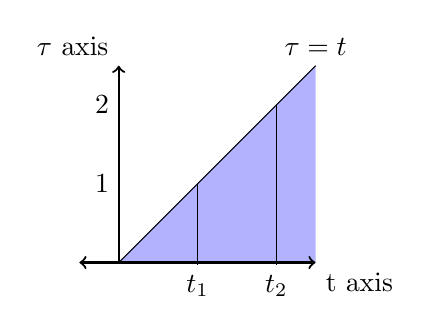
\begin{tikzpicture}
					\centering
					\fill[blue!30!white] (0,0) -- (2.5,2.5) -- (2.5,0) -- cycle;
					\draw[thick,<->] (-0.5,0) -- (2.5,0) node[anchor=north west] {t axis};
					\draw[thick,->] (0,0) -- (0,2.5) node[anchor=south east] {$\tau$ axis};
					\foreach \x in {1,2}
					\draw (\x cm,1pt) -- (\x cm,-1pt) node[anchor=north] {$t_{\x}$};
					\foreach \y in {1,2}
					\draw (0,\y cm) -- (0,\y cm) node[anchor=east] {$\y$};
					\draw[black] (0,0) -- (2.5,2.5) node[anchor=south] {$\tau = t$} ;
					\draw[black] (1,0) -- (1,1) ;
					\draw[black] (2,0) -- (2,2) ;
				\end{tikzpicture}
			\end{center}
			\caption{Before the change}
		\end{subfigure}%
		\begin{subfigure}{.4\textwidth}
			\begin{center}
				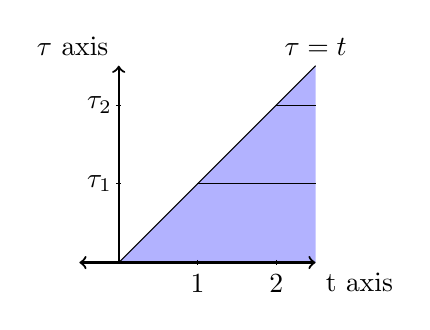
\begin{tikzpicture}
						\centering
						\fill[blue!30!white] (0,0) -- (2.5,2.5) -- (2.5,0) -- cycle;
						\draw[thick,<->] (-0.5,0) -- (2.5,0) node[anchor=north west] {t axis};
						\draw[thick,->] (0,0) -- (0,2.5) node[anchor=south east] {$\tau$ axis};
						\foreach \x in {1,2}
						\draw (\x cm,1pt) -- (\x cm,-1pt) node[anchor=north] {$\x$};
						\foreach \y in {1,2}
						\draw (-1pt,\y cm) -- (+1pt,\y cm) node[anchor=east] {$\tau_{\y}$};
						\draw[black] (0,0) -- (2.5,2.5) node[anchor=south] {$\tau = t$} ;
						\draw[black] (1,1) -- (2.5,1) ;
						\draw[black] (2,2) -- (2.5,2) ;
				\end{tikzpicture}
			\end{center}
			\caption{After the change}
		\end{subfigure}
		\caption{Visualisation of the change of limits }
		\label{fig:grenzenLaplace}
	\end{figure}
	\begin{equation}
		\left\{ \begin{array}{r@{\text{ $\rightarrow$ }}l}
			\tau:0&t \\
			 t:0&+\infty 
		\end{array}\right.\quad\Rightarrow\quad
	\left\{ \begin{array}{r@{\text{ $\rightarrow$ }}l}
		\tau:0&+\infty\\
		t:\tau&+\infty 
	\end{array}\right.
	\label{eq:Grenzen}
	\end{equation}
	We can now use a property of the exponential function:
	\begin{equation*}
		=\int_{0}^{+\infty}f(\tau)\left[ \int_{\tau}^{+\infty}g(t-\tau)\underbrace{e^{-s(t-\tau)}e^{-s\tau}}_{e^{-st}}dt\right]d\tau 
	\end{equation*}
	Then we apply the linearity property of integrals. Because of this, we can move the term $e^{-s\tau}$ outside of the inside integral.
	\begin{equation*}
		=\int_{0}^{+\infty}f(\tau)e^{-s\tau}\left[ \int_{\tau}^{+\infty}g(t-\tau)e^{-s(t-\tau)}dt\right] d\tau
	\end{equation*}%
	\newpage%
	We now use a substitution: $u = t-\tau  \Rightarrow du = dt \Rightarrow u: 0\rightarrow+\infty$
	\begin{equation*}
		=\int_{0}^{+\infty}f(\tau)e^{-s\tau}\left[ \underbrace{\int_{0}^{+\infty}g(u)e^{-su}du}_{=G(s)}\right] d\tau
	\end{equation*}
	We apply the linearity property of integrals for the final time to move $G(s)$ outside of the integral:
	\begin{align*}
		&=G(s)\underbrace{\int_{0}^{+\infty}f(\tau)e^{-s\tau}d\tau}_{=F(s)}\\
		&=G(s)\cdot F(s)
	\end{align*}
	Hereby we have proved that $f(t)\ast g(t)$ is equal to $F(s)\cdot G(s)$.
\end{document}
